\documentclass [a4paper,11pt]{article}
\usepackage{amssymb}
\usepackage{amsthm}
\usepackage[intlimits]{amsmath}
\usepackage[polish]{babel}
\usepackage[utf8]{inputenc}
\usepackage[T1]{fontenc}
\frenchspacing
\usepackage{indentfirst}
\usepackage{graphicx}
\usepackage{subfig}
\usepackage{mathptmx}
\usepackage{geometry}
\usepackage{wrapfig}
\usepackage{float}

\sloppy

\usepackage{array}
\newcolumntype{L}[1]{>{\raggedright\let\newline\\\arraybackslash\hspace{0pt}}m{#1}}
\newcolumntype{C}[1]{>{\centering\let\newline\\\arraybackslash\hspace{0pt}}m{#1}}
\newcolumntype{R}[1]{>{\raggedleft\let\newline\\\arraybackslash\hspace{0pt}}m{#1}}
\begin{document}
\newgeometry{tmargin=2cm, bmargin=2cm, lmargin=2cm, rmargin=2cm}

%----------- tabela nagłówkowa---------------------- %
\begin{table}[]
\centering
\begin{tabular}{lllllll}
\cline{1-6}
\multicolumn{1}{|c|}{\begin{tabular}[c]{@{}c@{}}EAiIB\\ Informatyka\end{tabular}}              & \multicolumn{2}{l|}{\begin{tabular}[c]{@{}l@{}}Autor 1\\ Autor 2\end{tabular}}                                                                                                & \multicolumn{1}{c|}{\begin{tabular}[c]{@{}c@{}}Rok\\ II\end{tabular}}          & \multicolumn{1}{c|}{\begin{tabular}[c]{@{}c@{}}Grupa\\ V\end{tabular}}            & \multicolumn{1}{c|}{\begin{tabular}[c]{@{}c@{}}Zespół\\ II\end{tabular}}      &  \\ \cline{1-6}
\multicolumn{1}{|c|}{\begin{tabular}[c]{@{}c@{}}Pracownia\\ FIZYCZNA\\ WFiIS AGH\end{tabular}} & \multicolumn{4}{l|}{\begin{tabular}[c]{@{}l@{}}Temat:\\ \textbf{Mostek Wheatstone'a} \end{tabular}}                                                                                                                                                                                                                                            & \multicolumn{1}{l|}{\begin{tabular}[c]{@{}l@{}}nr ćwiczenia:\\ 32\end{tabular}} &  \\ \cline{1-6}
\multicolumn{1}{|l|}{\begin{tabular}[c]{@{}c@{}}Data wykonania:\\ 7.10.2015\end{tabular}}      & \multicolumn{1}{c|}{\begin{tabular}[c]{@{}c@{}}Data oddania:\\ 14.10.2015\end{tabular}} & \multicolumn{1}{l|}{\begin{tabular}[c]{@{}l@{}}Zwrot do poprawki:\\ \phantom{data poprawki}\end{tabular}} & \multicolumn{1}{l|}{\begin{tabular}[c]{@{}l@{}}Data oddania:\\  \phantom{data oddania}\end{tabular}} & \multicolumn{1}{l|}{\begin{tabular}[c]{@{}l@{}}Data zaliczenia:\\  \phantom{data zaliczenia}\end{tabular}} & \multicolumn{1}{l|}{\begin{tabular}[c]{@{}l@{}}OCENA:\\ \phantom{ocena}\end{tabular}}       &  \\ \cline{1-6}
                                                                                               &                                                                                         &                                                                                     &                                                                                &                                                                                   &                                                                               & 
\end{tabular}
\end{table}



\section{Cel ćwiczenia}


Praktyczne zastosowanie praw Kirchhoffa, sprawdzenie zależności określających opór zastępczy dla połączenia szeregowego i równoległego.

\section{Opis eksperymentu}

Przy przeprowadzaniu eksperymentu skorzystano z układu pomiarowego, którego schemat przedstawia rysunek (\ref{fig:schemat}). Pomiędzy punktami A i C znajduje się listwa z  drutem oporowym o znanej długości. $R_2$ jest opornikiem wzorcowym o regulowanej wartości oporu, a $R_x$ nieznanym oporem, którego wartość chcemy wyznaczyć. Zrównoważenie mostka polega na takim ustawieniu punktu D, aby dla zadanej wartości $R_2$ przez galwanometr nie płynął prąd.
\begin{figure} [H]
\centering
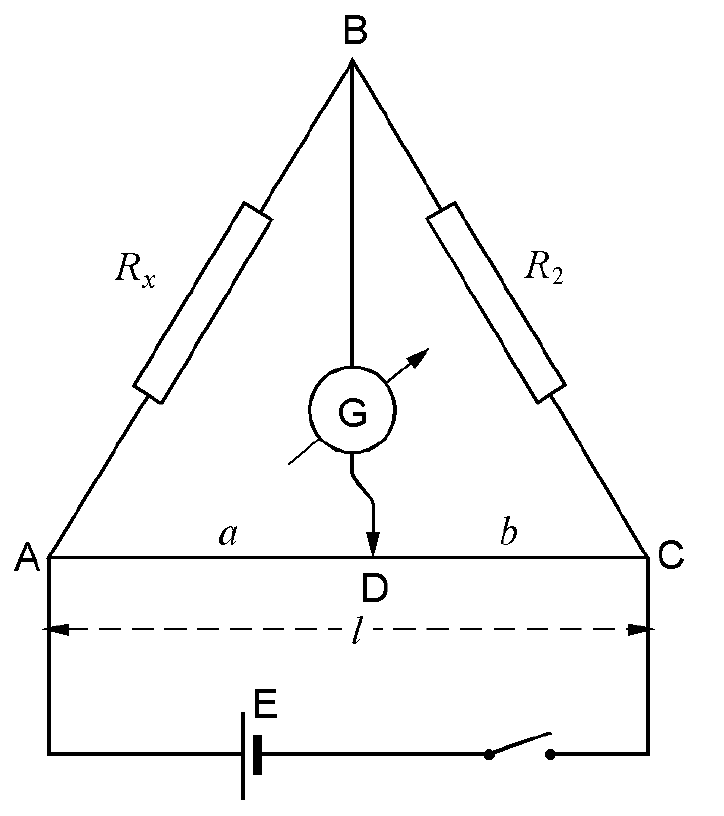
\includegraphics[width=0.4\linewidth]{./schemat}
\caption{Schemat mostka Wheatstone'a}
\label{fig:schemat}
\end{figure}


\section{Opracowanie wyników pomiarów}
Do obliczenia obliczenia nieznanej oporności $R_x$ na podstawie znanej oporności $R_2$ oraz zmierzonych długości $a$ i $l$  wykorzystujemy następujący wzór:

\begin{equation}
R_x = R_2 \frac{a}{l-a} \quad \text{gdzie: } \; l=1000mm
\label{eq:R_x} 
\end{equation}

Z kolei niepewność wartości $R_x$ jest wyznaczana z następującego wzoru:
\begin{equation}
u(R_x) = \sqrt{\frac{\sum_{i=1}^{n} \left( R_i - \overline{R_x} \right)^2 }{n(n-1)}}
\label{eq:R_x_delta} 
\end{equation}



\subsection{Opracowanie bezpośrednich wyników pomiarów}
\begin{table}[H]
\centering
\begin{tabular}{|l|r|r|r|r|r|r|r|r|r|r|}
\hline
$R_2[\Omega]$  & 14    & 20   & 16    & 18    & 10   & 12   & 8    & 7     & 5     & 22    \\
\hline
a[mm]  & 437   & 311  & 395   & 372   & 495  & 441  & 538  & 597   & 673   & 325   \\
\hline
$R_{x_1}$ & 10,87 & 9,03 & 10,45 & 10,66 & 9,80 & 9,47 & 9,32 & 10,37 & 10,29 & 10,59\\
\hline                      
\end{tabular}
\caption{Pomiary dla opornika $R_{x_1}$}
\label{tab:Rx1}
\end{table}

\begin{equation}
\overline{ R_{x_1}} = 10,08 [\Omega]
\label{eq:R_x1śr} 
\end{equation}

\begin{equation}
u(R_{x_1}) = 0,20 [\Omega]
\label{eq:R_x1_delta} 
\end{equation}



\begin{table}[H]
\centering
\begin{tabular}{|l|r|r|r|r|r|r|r|r|r|r|}
\hline
$R_2[\Omega]$ & 50    & 40    & 54    & 58    & 64    & 68    & 72    & 76    & 44    & 48    \\
\hline
a[mm]  & 466   & 525   & 453   & 435   & 411   & 394   & 374   & 365   & 505   & 480   \\
\hline
$R_{x_2}[\Omega]$& 43,63 & 44,21 & 44,72 & 44,65 & 44,66 & 44,21 & 43,02 & 43,69 & 44,89 & 44,31 \\
\hline
\end{tabular}
\caption{Pomiary dla opornika $R_{x_2}$}
\label{tab:Rx2}
\end{table}


\begin{equation}
\overline{ R_{x_2}} = 44,20 [\Omega]
\label{eq:R_x2śr} 
\end{equation}

\begin{equation}
u(R_{x_2}) = 0,19 [\Omega]
\label{eq:R_x2_delta} 
\end{equation}

\begin{table}[H]
\centering
\begin{tabular}{|l|r|r|r|r|r|r|r|r|r|r|}
\hline
$R_2[\Omega]$   & 60    & 70    & 80    & 90    & 50    & 40    & 45    & 55    & 65    & 75    \\
\hline
a[mm]   & 460   & 430   & 398   & 370   & 512   & 575   & 545   & 496   & 458   & 422   \\
\hline
$R_{x_{12\text{szer}}}[\Omega]$  & 51,11 & 52,81 & 52,89 & 52,86 & 52,46 & 54,12 & 53,90 & 54,13 & 54,93 & 54,76 \\
\hline
\end{tabular}
\caption{Pomiary dla połączenia szeregowego oporników $R_{x_2}$ i $R_{x_1}$}
\label{tab:Rx12szer}
\end{table}

\begin{equation}
\overline{R_{x_{12\text{szer}}}} = 53,40 [\Omega]
\label{eq:R_x12szer_śr} 
\end{equation}

\begin{equation}
u(R_{x_{12\text{szer}}}) = 0,38 [\Omega]
\label{eq:R_x12szer_delta} 
\end{equation}

\begin{table}[H]
\centering
\begin{tabular}{|l|r|r|r|r|r|r|r|r|r|r|}
\hline
$R_2[\Omega]$    & 6    & 7    & 8    & 9    & 10   & 11   & 12   & 13   & 14   & 15   \\
\hline
a[mm]    & 600  & 555  & 529  & 495  & 466  & 435  & 412  & 403  & 391  & 378  \\
\hline
$R_{x_{12\text{rów}}}[\Omega]$& 9,00 & 8,73 & 8,99 & 8,82 & 8,73 & 8,47 & 8,41 & 8,78 & 8,99 & 9,12 \\
\hline
\end{tabular}
\caption{Pomiary dla połączenia równoległego oporników $R_{x_2}$ i $R_{x_1}$}
\label{tab:Rx12row}
\end{table}

\begin{equation}
\overline{R_{x_{12\text{rów}}}} = 8,80 [\Omega]
\label{eq:R_x12rów_śr} 
\end{equation}

\begin{equation}
u(R_{x_{12\text{rów}}}) = 0,08 [\Omega]
\label{eq:R_x12row_delta} 
\end{equation}

\subsection{Połączenie szeregowe}
Wartość oporu przy połączeniu szeregowym można też obliczyć na podstawie wzoru na opór zastępczy oraz wyznaczonych wartości $R_{x_1}$ i  $R_{x_2}$

\begin{equation}
R_{z_{szer}} = R_{x_1} + R_{x_2} = 54,28 [\Omega]
\label{eq:R_x12szer_zast} 
\end{equation}

\begin{equation}
u(R_{z_{szer}}) = \sqrt{\left( \frac{\delta R_{z_{szer}} }{\delta R_{x_1}}  \right)^2 u(R_{x_1})^2  +\left( \frac{\delta R_{z_{szer}} }{\delta R_{x_2}}  \right)^2  u(R_{x_2})^2  }  = \sqrt{u(R_{x_1})^2 + u(R_{x_2})^2} =  0,28 [\Omega]
\label{eq:R_x12szer_zast_delta} 
\end{equation}

\subsection{Połączenie równoległe}
Wartość oporu przy połączeniu równoległym można też obliczyć na podstawie wzoru na opór zastępczy oraz wyznaczonych wartości $R_{x_1}$ i  $R_{x_2}$
\begin{equation}
R_{z_\text{rów}} = \frac{ R_{x_1} R_{x_2}}{ R_{x_1} + R_{x_2}} = 8,21 [\Omega]
\label{eq:R_x12row_zast} 
\end{equation}

\begin{multline}
u(R_{z_\text{rów}}) = \sqrt{\left( \frac{\delta R_{z_\text{rów}} }{\delta R_{x_1}}  \right)^2 u(R_{x_1})^2  +\left( \frac{\delta R_{z_\text{rów}} }{\delta R_{x_2}}  \right)^2  u(R_{x_2})^2  }  = \\ \sqrt{\left(  \frac{R_{x_1}}{R_{x_1} + R_{x_2}}\right)^4  u(R_{x_1})^2 + \left(\frac{R_{x_2}}{R_{x_1} + R_{x_2}}\right)^4  u(R_{x_2})^2   } =  0,13 [\Omega]
\label{eq:R_x12row_zast_delta} 
\end{multline}

\subsection{Porównanie wartości z pomiarów i wyznaczonych ze wzorów}
\begin{tabular}{|c|c|c|}
\hline 						 & R wyznaczone [$\Omega$]  & R obliczone [$\Omega$] \\ 
\hline Połączenie szeregowe & $53,40 \pm 0,38$ & $54,28 \pm 0,28$ \\ 
\hline Połączenie równoległe & $8,80 \pm 0,08$ & $8,21 \pm 0,13$ \\ 
\hline 
\end{tabular} 
\section{Wnioski}
\begin{itemize}
%\item Niepewności przy eksperymentalnym wyznaczaniu oporności są dosyć małe, co świadczy o dokładności metody. 
\item W przypadku połączenia szeregowego wartości uzyskane doświadczalnie i obliczone ze wzoru na opór zastępczy są ze sobą zgodne w granicach niepewności pomiarowych(biorąc pod uwagę niepewność rozszerzoną). W przypadku połączenia równoległego wartości te nie są zgodne.
\item Wpływ na niedokładność wyników mógł mieć fakt, iż drut oporowy nie był idealnie prosty i naciągnięty, co wpływało na wartość pomiarów na nim wykonywanych.
 
\end{itemize}

\end{document}